{\textbf{1. 将树转换为二叉树}}

{{步骤1:加线。}在各兄弟结点之间用虚线相连。可理解为每个结点的兄弟指针指向它的一个兄弟。}

{{步骤2:}{删除线。}对每个结点仅保留它与其最左一个孩子的连线,删除该结点与其他孩子之间的连线。可理解为每个结点仅有一个孩子指针,让它指向自己的长子。}

{{步骤3:旋转。}把虚线改为实线从水平方向向下旋转45度,成右斜下方向。原树中实线如左斜下方向。这样就树的形状成呈现出一棵二叉树。}

{下图中a所示的树,可转换为图中d所示的二叉树。}

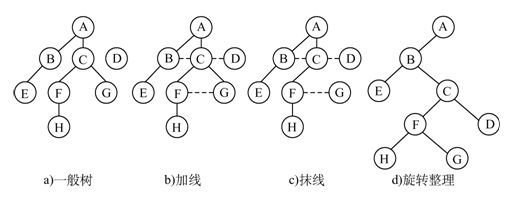
\includegraphics[width=3.70833in,height=1.45833in]{png-jpeg-pics/47A9E641635D85EE843D278FDFA2CB04.png}

{\textbf{2. 将一个森林转换为二叉树}}

{森林是树的有限集合,如下图a所示。由上节可知,一棵树可以转换为二叉树(没有右子树),一个森林就可以转换为二叉树(没有右子树)的森林。将森林转换为二叉树的一般步骤为:}

{{步骤1:}将森林中每棵子树转换成相应的二叉树。形成有若干二叉树的森林,如下图b所示。}

{{步骤2:}按森林图形中树的先后次序,依次将后边一棵二叉树作为前边一棵二叉树根结点的右子树,这样整个森林就生成了一棵二叉树,实际上第一棵树的根结点便是生成后的二叉树的根结点。下图是将一个森林转化为一棵二叉树的示例。图中d是转化后的一棵二叉树。下图中,图中a包含三棵树的森林可转换为图中d所示的二叉树。}

{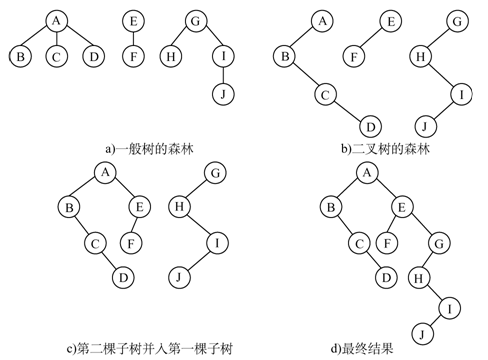
\includegraphics[width=3.70833in,height=2.73958in]{png-jpeg-pics/8E1BB4B1D59EC35B61044A5A4531A9DF.png}\\
}

{\textbf{3. 二叉树转换为一般树}}

{此时的二叉树必须是由某一树(一般树)转换而来的没有右子树的二叉树。并非随便一棵二叉树都能还原成一般树。}

{其还原过程也分为三步:}

{{步骤1:加线。}若某结点i是双亲结点的左孩子,则将该结点i的右孩子以及当且仅当连续地沿着右孩子的右链不断搜索到所有右孩子,都分别与结点i的双亲结点用虚线连接。}

{{步骤2:删除线。}把原二叉树中所有双亲结点与其右孩子的连线删除。这里的右孩子实质上是原一般树中结点的兄弟,删除的连线是兄弟间的关系。}

{{步骤3:进行整理。}把虚线改为实线,把结点按层次排列。}

{下图是把二叉树还原为一般树。}

{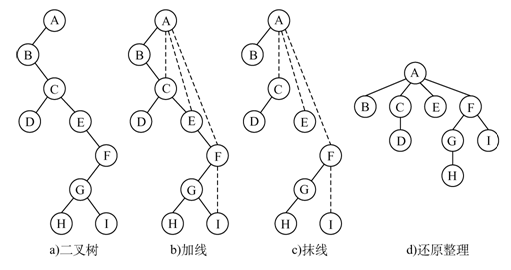
\includegraphics[width=3.70833in,height=1.95833in]{png-jpeg-pics/61F1D65B8B45C7E8E61FD9B3735B636C.png}\\
}

{}

{\textbf{4. 二叉树转换为森林}}

{将一棵二叉树转化成森林,可按如下步骤进行:}

{删除线:将二叉树根结点与其右孩子之间的连线,以及沿着此右孩子的右链连续不断搜索到的右孩子间的连线删除。这样就得到了若干棵根结点没有右子树的二叉树。将得到的这些二叉树用前述方法分别转化成一般树。}
